\documentclass{article}

\usepackage[utf8]{inputenc}
\usepackage[english]{babel}

\usepackage{amsmath,amsfonts,amssymb}
\usepackage{fullpage}
\usepackage{verbatim}

\usepackage{tikz,pgfplots}

\pgfplotsset{
    width=160mm,height=150mm,
    major grid style={thin,dotted,color=black!50},
    minor grid style={thin,dotted,color=black!50},
    grid,
    every axis/.append style={
        line width=0.5pt,
        tick style={
            line cap=round,
            thin,
            major tick length=4pt,
            minor tick length=2pt,
        },
    },
    legend cell align=left,
    legend pos=north west,
}

%%%%%%%%%%%%%%%%%%%%%%%%%%%%%%%%%%%%%%%%%%%%%%%%%%%%%%%%%%%%%%%%%%%%%%%%%%%%%%%%

\begin{document}

\section{Construction times and memory utilization}
% IMPORT-DATA stats sqlplot.txt

\begin{center}
    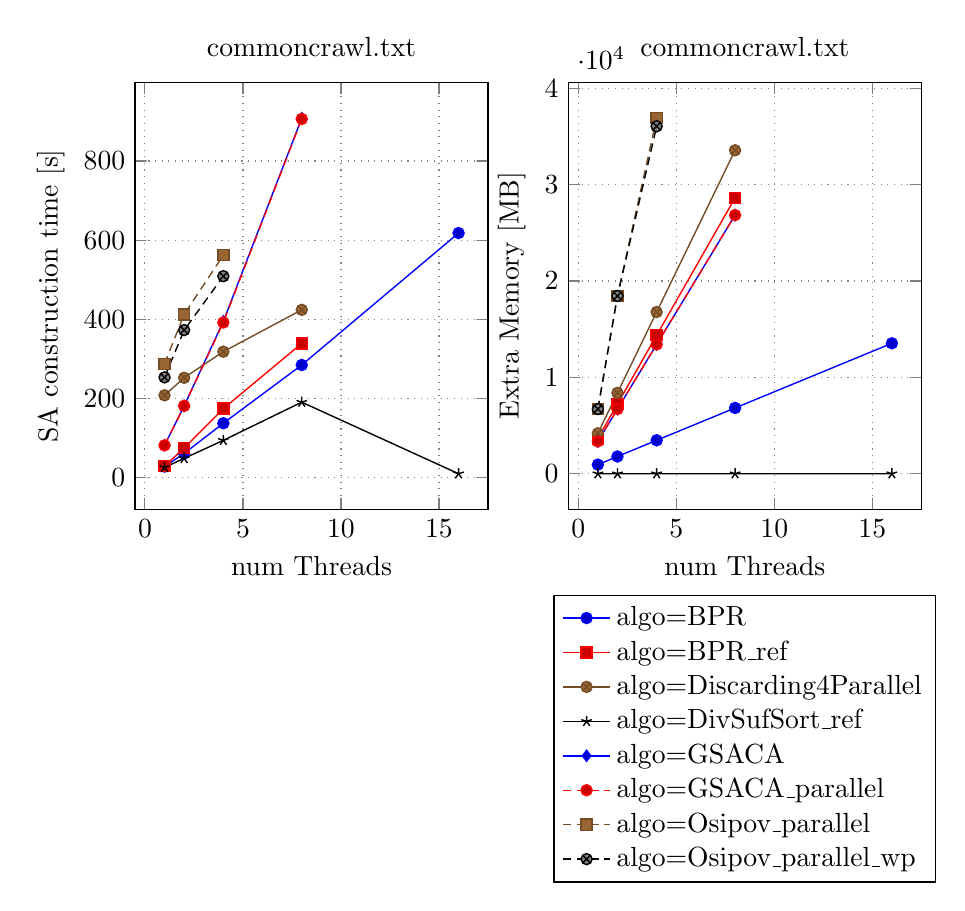
\begin{tikzpicture}
        \begin{axis}[
                name=axis1,
                width=0.5\textwidth,
                height=70mm,
                title={commoncrawl.txt},
                xlabel={num Threads},
                ylabel={SA construction time [s]},
            ]

            %% MULTIPLOT(algo) SELECT threads AS x, time/1000 AS y, MULTIPLOT
            %% FROM stats WHERE rep_i=0 AND input="commoncrawl.txt" AND NOT algo="Deep-Shallow_par" GROUP BY MULTIPLOT,x ORDER BY MULTIPLOT,x
            \addplot coordinates { (1,28.2981) (2,61.3645) (4,137.674) (8,284.744) (16,618.018) };
            \addlegendentry{algo=BPR};
            \addplot coordinates { (1,29.6373) (2,74.7488) (4,174.575) (8,339.26) };
            \addlegendentry{algo=BPR\_ref};
            \addplot coordinates { (1,208.234) (2,252.456) (4,318.425) (8,424.083) };
            \addlegendentry{algo=Discarding4Parallel};
            \addplot coordinates { (1,26.1582) (2,48.8489) (4,94.515) (8,190.863) (16,10.1305) };
            \addlegendentry{algo=DivSufSort\_ref};
            \addplot coordinates { (1,81.8306) (2,181.533) (4,394.937) (8,908.134) };
            \addlegendentry{algo=GSACA};
            \addplot coordinates { (1,81.8237) (2,181.486) (4,392.112) (8,906.325) };
            \addlegendentry{algo=GSACA\_parallel};
            \addplot coordinates { (1,287.845) (2,412.553) (4,562.45) };
            \addlegendentry{algo=Osipov\_parallel};
            \addplot coordinates { (1,253.517) (2,372.944) (4,509.089) };
            \addlegendentry{algo=Osipov\_parallel\_wp};

            \legend{}
        \end{axis}
        \begin{axis}[
                at={(axis1.outer north east)},
                anchor=outer north west,
                name=axis2,
                width=0.5\textwidth,
                height=70mm,
                title={commoncrawl.txt},
                xlabel={num Threads},
                ylabel={Extra Memory [MB]},
                legend style={at={(0.5, -0.2)}, anchor=north},
            ]

            %% MULTIPLOT(algo) SELECT threads AS x, memPeak/1000000 AS y, MULTIPLOT
            %% FROM (
            %% SELECT algo, input, MEDIAN(memFinal) AS memFinal, MEDIAN(memOff) AS memOff, AVG(memPeak) AS memPeak, prefix, rep, threads, MEDIAN(time) AS time FROM stats GROUP BY algo, input, prefix, rep, threads
            %% ) WHERE input="commoncrawl.txt" AND NOT algo="Deep-Shallow_par" GROUP BY MULTIPLOT,x ORDER BY MULTIPLOT,x
            \addplot coordinates { (1,944.015) (2,1789.7) (4,3470.23) (8,6825.68) (16,13536.6) };
            \addlegendentry{algo=BPR};
            \addplot coordinates { (1,3668.99) (2,7240.91) (4,14374) (8,28634.7) };
            \addlegendentry{algo=BPR\_ref};
            \addplot coordinates { (1,4196.45) (2,8393) (4,16785.9) (8,33571.7) };
            \addlegendentry{algo=Discarding4Parallel};
            \addplot coordinates { (1,0.264792) (2,0.264029) (4,0.264573) (8,0.265661) (16,0.0) };
            \addlegendentry{algo=DivSufSort\_ref};
            \addplot coordinates { (1,3355.45) (2,6710.89) (4,13421.8) (8,26843.5) };
            \addlegendentry{algo=GSACA};
            \addplot coordinates { (1,3355.45) (2,6710.89) (4,13421.8) (8,26843.6) };
            \addlegendentry{algo=GSACA\_parallel};
            \addplot coordinates { (1,6709.8) (2,18450.3) (4,36903.6) };
            \addlegendentry{algo=Osipov\_parallel};
            \addplot coordinates { (1,6709.8) (2,18450.3) (4,36065) };
            \addlegendentry{algo=Osipov\_parallel\_wp};

        \end{axis}
    \end{tikzpicture}
\end{center}

\begin{center}
    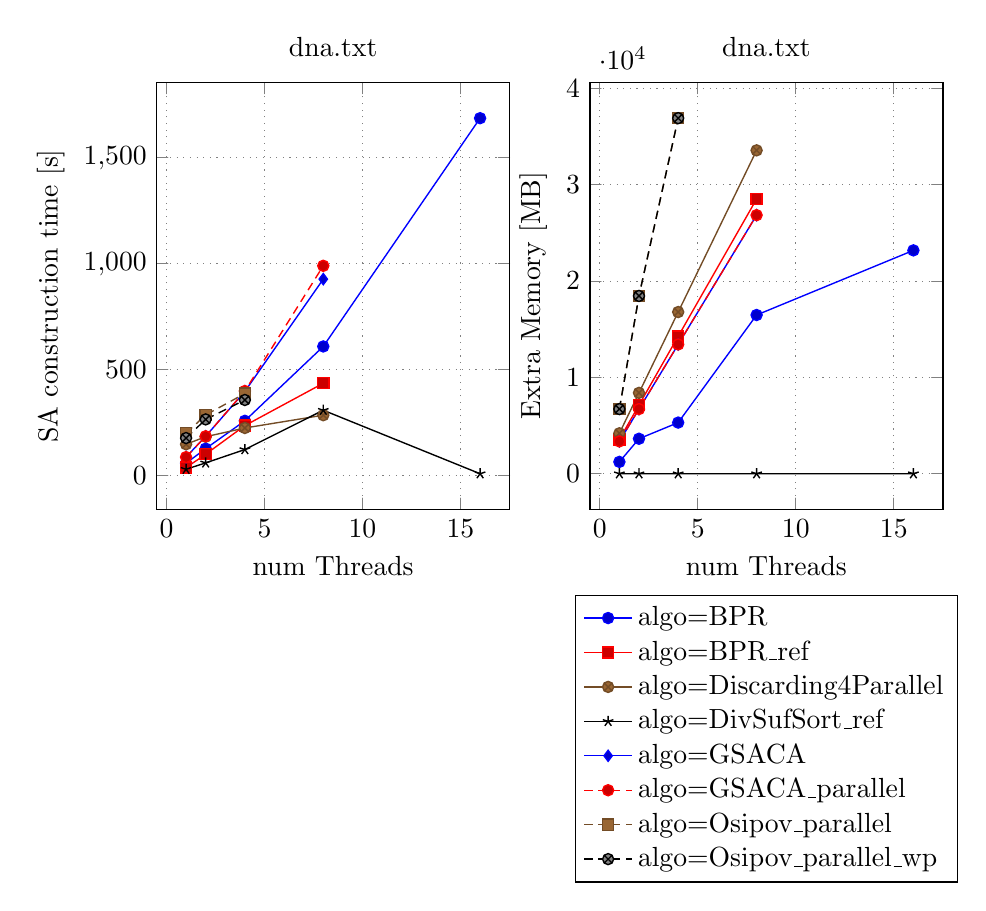
\begin{tikzpicture}
        \begin{axis}[
                name=axis1,
                width=0.5\textwidth,
                height=70mm,
                title={dna.txt},
                xlabel={num Threads},
                ylabel={SA construction time [s]},
            ]

            %% MULTIPLOT(algo) SELECT threads AS x, time/1000 AS y, MULTIPLOT
            %% FROM stats WHERE rep_i=0 AND input="dna.txt" AND NOT algo="Deep-Shallow_par" GROUP BY MULTIPLOT,x ORDER BY MULTIPLOT,x
            \addplot coordinates { (1,59.4033) (2,128.075) (4,259.353) (8,610.115) (16,1686.72) };
            \addlegendentry{algo=BPR};
            \addplot coordinates { (1,38.5197) (2,101.598) (4,236.856) (8,436.506) };
            \addlegendentry{algo=BPR\_ref};
            \addplot coordinates { (1,148.773) (2,184.372) (4,225.571) (8,285.869) };
            \addlegendentry{algo=Discarding4Parallel};
            \addplot coordinates { (1,30.9183) (2,60.9494) (4,123.84) (8,309.275) (16,9.81616) };
            \addlegendentry{algo=DivSufSort\_ref};
            \addplot coordinates { (1,88.2974) (2,186.423) (4,398.098) (8,927.613) };
            \addlegendentry{algo=GSACA};
            \addplot coordinates { (1,88.1879) (2,186.338) (4,399.907) (8,990.527) };
            \addlegendentry{algo=GSACA\_parallel};
            \addplot coordinates { (1,200.778) (2,287.025) (4,388.067) };
            \addlegendentry{algo=Osipov\_parallel};
            \addplot coordinates { (1,178.085) (2,265.998) (4,357.599) };
            \addlegendentry{algo=Osipov\_parallel\_wp};

            \legend{}
        \end{axis}
        \begin{axis}[
                at={(axis1.outer north east)},
                anchor=outer north west,
                name=axis2,
                width=0.5\textwidth,
                height=70mm,
                title={dna.txt},
                xlabel={num Threads},
                ylabel={Extra Memory [MB]},
                legend style={at={(0.5, -0.2)}, anchor=north},
            ]

            %% MULTIPLOT(algo) SELECT threads AS x, memPeak/1000000 AS y, MULTIPLOT
            %% FROM (
            %% SELECT algo, input, MEDIAN(memFinal) AS memFinal, MEDIAN(memOff) AS memOff, AVG(memPeak) AS memPeak, prefix, rep, threads, MEDIAN(time) AS time FROM stats GROUP BY algo, input, prefix, rep, threads
            %% ) WHERE input="dna.txt" AND NOT algo="Deep-Shallow_par" GROUP BY MULTIPLOT,x ORDER BY MULTIPLOT,x
            \addplot coordinates { (1,1229.49) (2,3630.85) (4,5308.57) (8,16476.5) (16,23187.4) };
            \addlegendentry{algo=BPR};
            \addplot coordinates { (1,3565.29) (2,7130.45) (4,14260.8) (8,28521.4) };
            \addlegendentry{algo=BPR\_ref};
            \addplot coordinates { (1,4196.45) (2,8393) (4,16785.9) (8,33571.7) };
            \addlegendentry{algo=Discarding4Parallel};
            \addplot coordinates { (1,0.264792) (2,0.264029) (4,0.264573) (8,0.265661) (16,0.0) };
            \addlegendentry{algo=DivSufSort\_ref};
            \addplot coordinates { (1,3355.44) (2,6710.89) (4,13421.8) (8,26843.5) };
            \addlegendentry{algo=GSACA};
            \addplot coordinates { (1,3355.44) (2,6710.89) (4,13421.8) (8,26843.5) };
            \addlegendentry{algo=GSACA\_parallel};
            \addplot coordinates { (1,6710.89) (2,18454.9) (4,36909.9) };
            \addlegendentry{algo=Osipov\_parallel};
            \addplot coordinates { (1,6710.89) (2,18454.9) (4,36909.9) };
            \addlegendentry{algo=Osipov\_parallel\_wp};

        \end{axis}
    \end{tikzpicture}
\end{center}

\section{Example: 4 plots aligned}
\begin{center}
    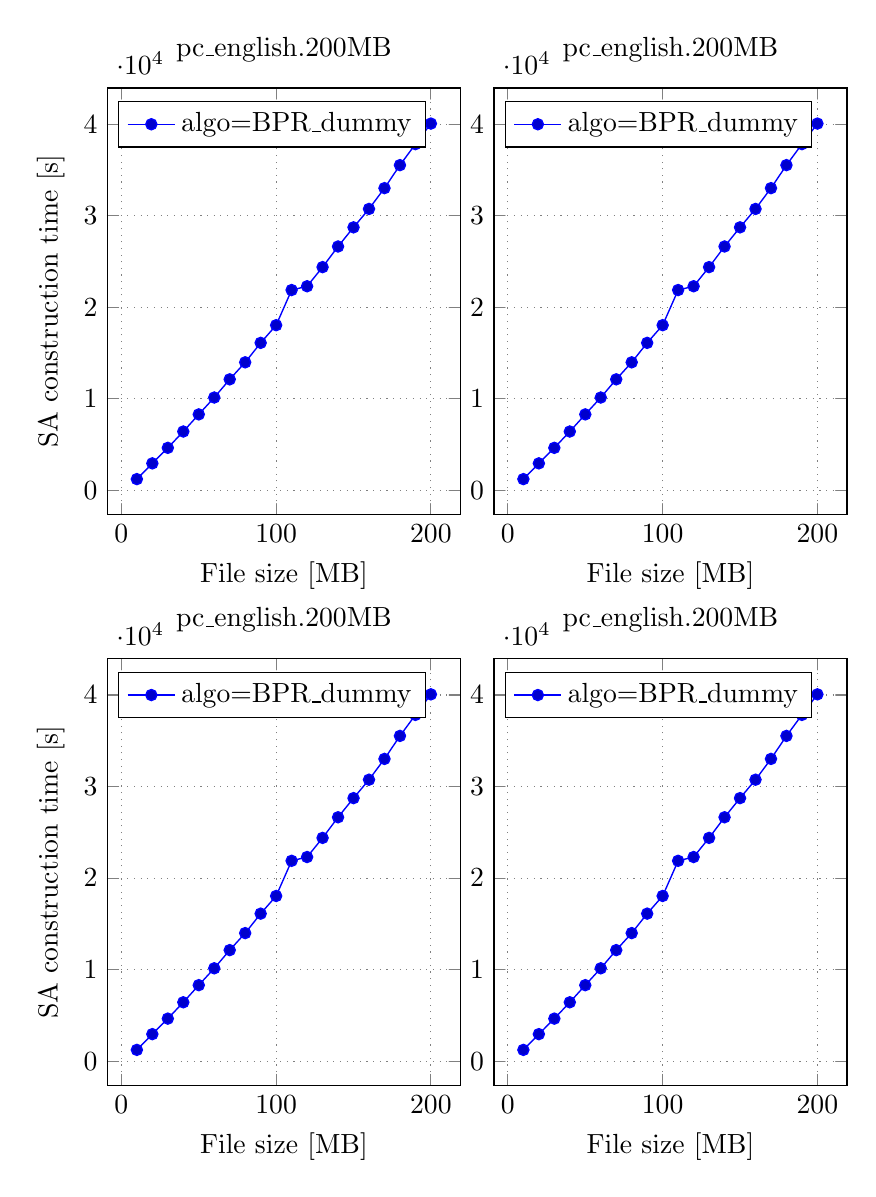
\begin{tikzpicture}
        \begin{axis}[
                name=axis1,
                width=0.5\textwidth,
                height=70mm,
                title={pc\_english.200MB},
                xlabel={File size [MB]},
                ylabel={SA construction time [s]},
            ]

            %% MULTIPLOT(algo) SELECT prefix/1000000 AS x, time AS y, MULTIPLOT
            %% FROM stats WHERE algo="BPR_dummy" GROUP BY MULTIPLOT,x ORDER BY MULTIPLOT,x
            \addplot coordinates { (10,1234.0) (20,2954.0) (30,4649.0) (40,6433.0) (50,8303.0) (60,10145.0) (70,12131.0) (80,13990.0) (90,16116.0) (100,18045.0) (110,21886.0) (120,22299.0) (130,24388.0) (140,26642.0) (150,28733.0) (160,30743.0) (170,33016.0) (180,35528.0) (190,37823.0) (200,40068.0) };
            \addlegendentry{algo=BPR\_dummy};

        \end{axis}
        \begin{axis}[
                at={(axis1.outer north east)},
                anchor=outer north west,
                name=axis2,
                width=0.5\textwidth,
                height=70mm,
                title={pc\_english.200MB},
                xlabel={File size [MB]},
            ]

            %% MULTIPLOT(algo) SELECT prefix/1000000 AS x, time AS y, MULTIPLOT
            %% FROM stats WHERE algo="BPR_dummy" GROUP BY MULTIPLOT,x ORDER BY MULTIPLOT,x
            \addplot coordinates { (10,1234.0) (20,2954.0) (30,4649.0) (40,6433.0) (50,8303.0) (60,10145.0) (70,12131.0) (80,13990.0) (90,16116.0) (100,18045.0) (110,21886.0) (120,22299.0) (130,24388.0) (140,26642.0) (150,28733.0) (160,30743.0) (170,33016.0) (180,35528.0) (190,37823.0) (200,40068.0) };
            \addlegendentry{algo=BPR\_dummy};

        \end{axis}
        \begin{axis}[
                at={(axis1.outer south west)},
                anchor=outer north west,
                name=axis3,
                width=0.5\textwidth,
                height=70mm,
                title={pc\_english.200MB},
                xlabel={File size [MB]},
                ylabel={SA construction time [s]},
            ]

            %% MULTIPLOT(algo) SELECT prefix/1000000 AS x, time AS y, MULTIPLOT
            %% FROM stats WHERE algo="BPR_dummy" GROUP BY MULTIPLOT,x ORDER BY MULTIPLOT,x
            \addplot coordinates { (10,1234.0) (20,2954.0) (30,4649.0) (40,6433.0) (50,8303.0) (60,10145.0) (70,12131.0) (80,13990.0) (90,16116.0) (100,18045.0) (110,21886.0) (120,22299.0) (130,24388.0) (140,26642.0) (150,28733.0) (160,30743.0) (170,33016.0) (180,35528.0) (190,37823.0) (200,40068.0) };
            \addlegendentry{algo=BPR\_dummy};

        \end{axis}
        \begin{axis}[
                at={(axis3.outer north east)},
                anchor=outer north west,
                name=axis4,
                width=0.5\textwidth,
                height=70mm,
                title={pc\_english.200MB},
                xlabel={File size [MB]},
            ]

            %% MULTIPLOT(algo) SELECT prefix/1000000 AS x, time AS y, MULTIPLOT
            %% FROM stats WHERE algo="BPR_dummy" GROUP BY MULTIPLOT,x ORDER BY MULTIPLOT,x
            \addplot coordinates { (10,1234.0) (20,2954.0) (30,4649.0) (40,6433.0) (50,8303.0) (60,10145.0) (70,12131.0) (80,13990.0) (90,16116.0) (100,18045.0) (110,21886.0) (120,22299.0) (130,24388.0) (140,26642.0) (150,28733.0) (160,30743.0) (170,33016.0) (180,35528.0) (190,37823.0) (200,40068.0) };
            \addlegendentry{algo=BPR\_dummy};

        \end{axis}
    \end{tikzpicture}
\end{center}

\section{Extra memory usage}
\begin{center}
    \begin{tikzpicture}
        \begin{axis}[
                title={pc\_english.200MB},
                xlabel={File Size [Bytes]},
                ylabel={Extra Memory [Bytes]},
            ]

            %% MULTIPLOT(algo) SELECT prefix AS x, memPeak AS y, MULTIPLOT
            %% FROM stats WHERE algo="BPR_dummy" GROUP BY MULTIPLOT,x ORDER BY MULTIPLOT,x
            \addplot coordinates { (10000000,10000000) (1e+08,1e+08) (1.1e+08,1.1e+08) (1.2e+08,1.2e+08) (1.3e+08,1.3e+08) (1.4e+08,1.4e+08) (1.5e+08,1.5e+08) (1.6e+08,1.6e+08) (1.7e+08,1.7e+08) (1.8e+08,1.8e+08) (1.9e+08,1.9e+08) (20000000,20000000) (2e+08,2e+08) (30000000,30000000) (40000000,40000000) (50000000,50000000) (60000000,60000000) (70000000,70000000) (80000000,80000000) (90000000,90000000) };
            \addlegendentry{algo=BPR\_dummy};

        \end{axis}
    \end{tikzpicture}
\end{center}

\section{Extra memory per input byte}
\begin{center}
    \begin{tikzpicture}
        \begin{axis}[
                title={pc\_english.200MB},
                xlabel={File Size [MB]},
                ylabel={Extra Memory in Bytes per input Byte},
            ]

            %% MULTIPLOT(algo) SELECT prefix/1000000 AS x, memPeak/prefix AS y, MULTIPLOT
            %% FROM stats WHERE algo="BPR_dummy" GROUP BY MULTIPLOT,x ORDER BY MULTIPLOT,x
            \addplot coordinates { (10,1) (20,1) (30,1) (40,1) (50,1) (60,1) (70,1) (80,1) (90,1) (100,1) (110,1) (120,1) (130,1) (140,1) (150,1) (160,1) (170,1) (180,1) (190,1) (200,1) };
            \addlegendentry{algo=BPR\_dummy};

        \end{axis}
    \end{tikzpicture}
\end{center}

\end{document}

